In diesem Versuch nutzen wir eine Quecksilber-Franck-Hertz-Röhre um verschiedene Effekte zu untersuchen.
\begin{figure}
	\centering
	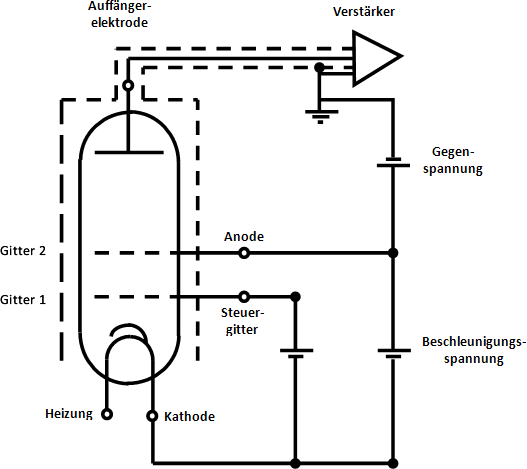
\includegraphics[width=0.5\textwidth]{../Daten/Aufgabe1/Aufbau.png}
	\caption{Skizze einer Franck-Hertz-Röhre \cite{FHR}}
\end{figure}
\section{Aufbau}
Bei der Franck-Hertz-Röhre handelt es sich um einen abgeschlossenen, mit Gas gefüllten Glaskörper. In diesem werden mithilfe einer Heizspirale freie Elektronen erzeugt, die dann mithilfe einer angelegten Spannung und eines Steuergitters beschleunigt werden. Auf der gegenüberliegenden Seite der Röhre befindet sich eine Auffangelektrode. Zwischen den beiden befindet sich ein Gitter, welches als Anode zur Heizspirale agiert. Zwischen Gitter und Auffangelektrode befindet sich ein schwaches Gegenfeld. Bei unserer Messung erwarten wir, dass wir mit steigender Beschleunigungsspannung eine zunehmende Anzahl von Elektronen bei der Auffangelektrode registrieren, wobei es allerdings in gleichbleibenden Abständen Abfälle gibt. Diese Form wird auch Franck-Herz-Kurve genannt. Um den Versuch durchzuführen bauten wir ihn zunächst wie in der Aufgabenstellung beschrieben auf.
\section{Bestimmung der Kontaktspannung zwischen Kathode und Anode}
Dann ermitteln wir die Thermokontaktspannung. Bei der Aufnahme der Daten haben wir leider Versäumt den Graphen der Messung bei 120$\; ^\circ $C abzuspeichern, weswegen für diesen nur die Daten ohne Bild vorliegen.
\begin{figure}
	\centering
	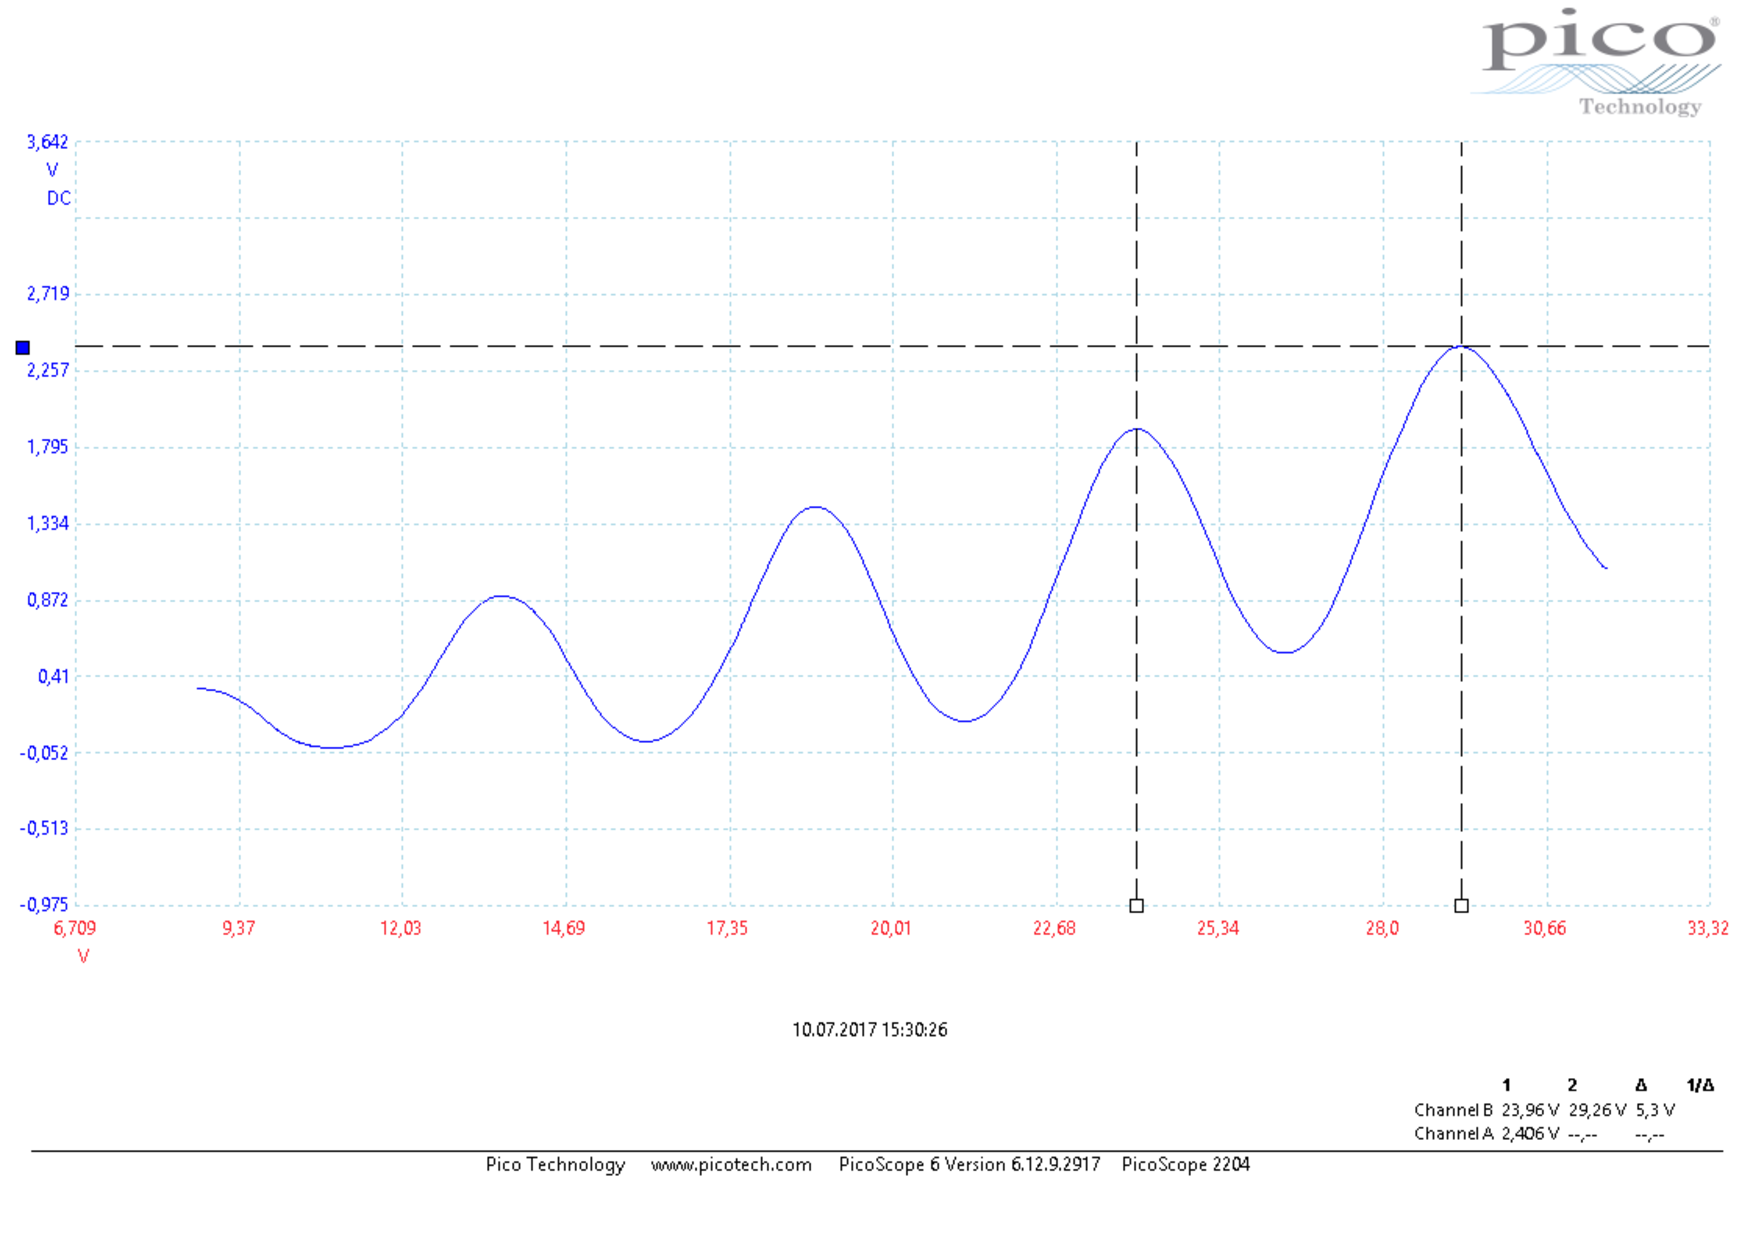
\includegraphics[width=\textwidth]{../Daten/Aufgabe1/Frank_Hertz_140.pdf}
	\caption{Franck-Herz-Kurve bei 140$ ^\circ $C}
	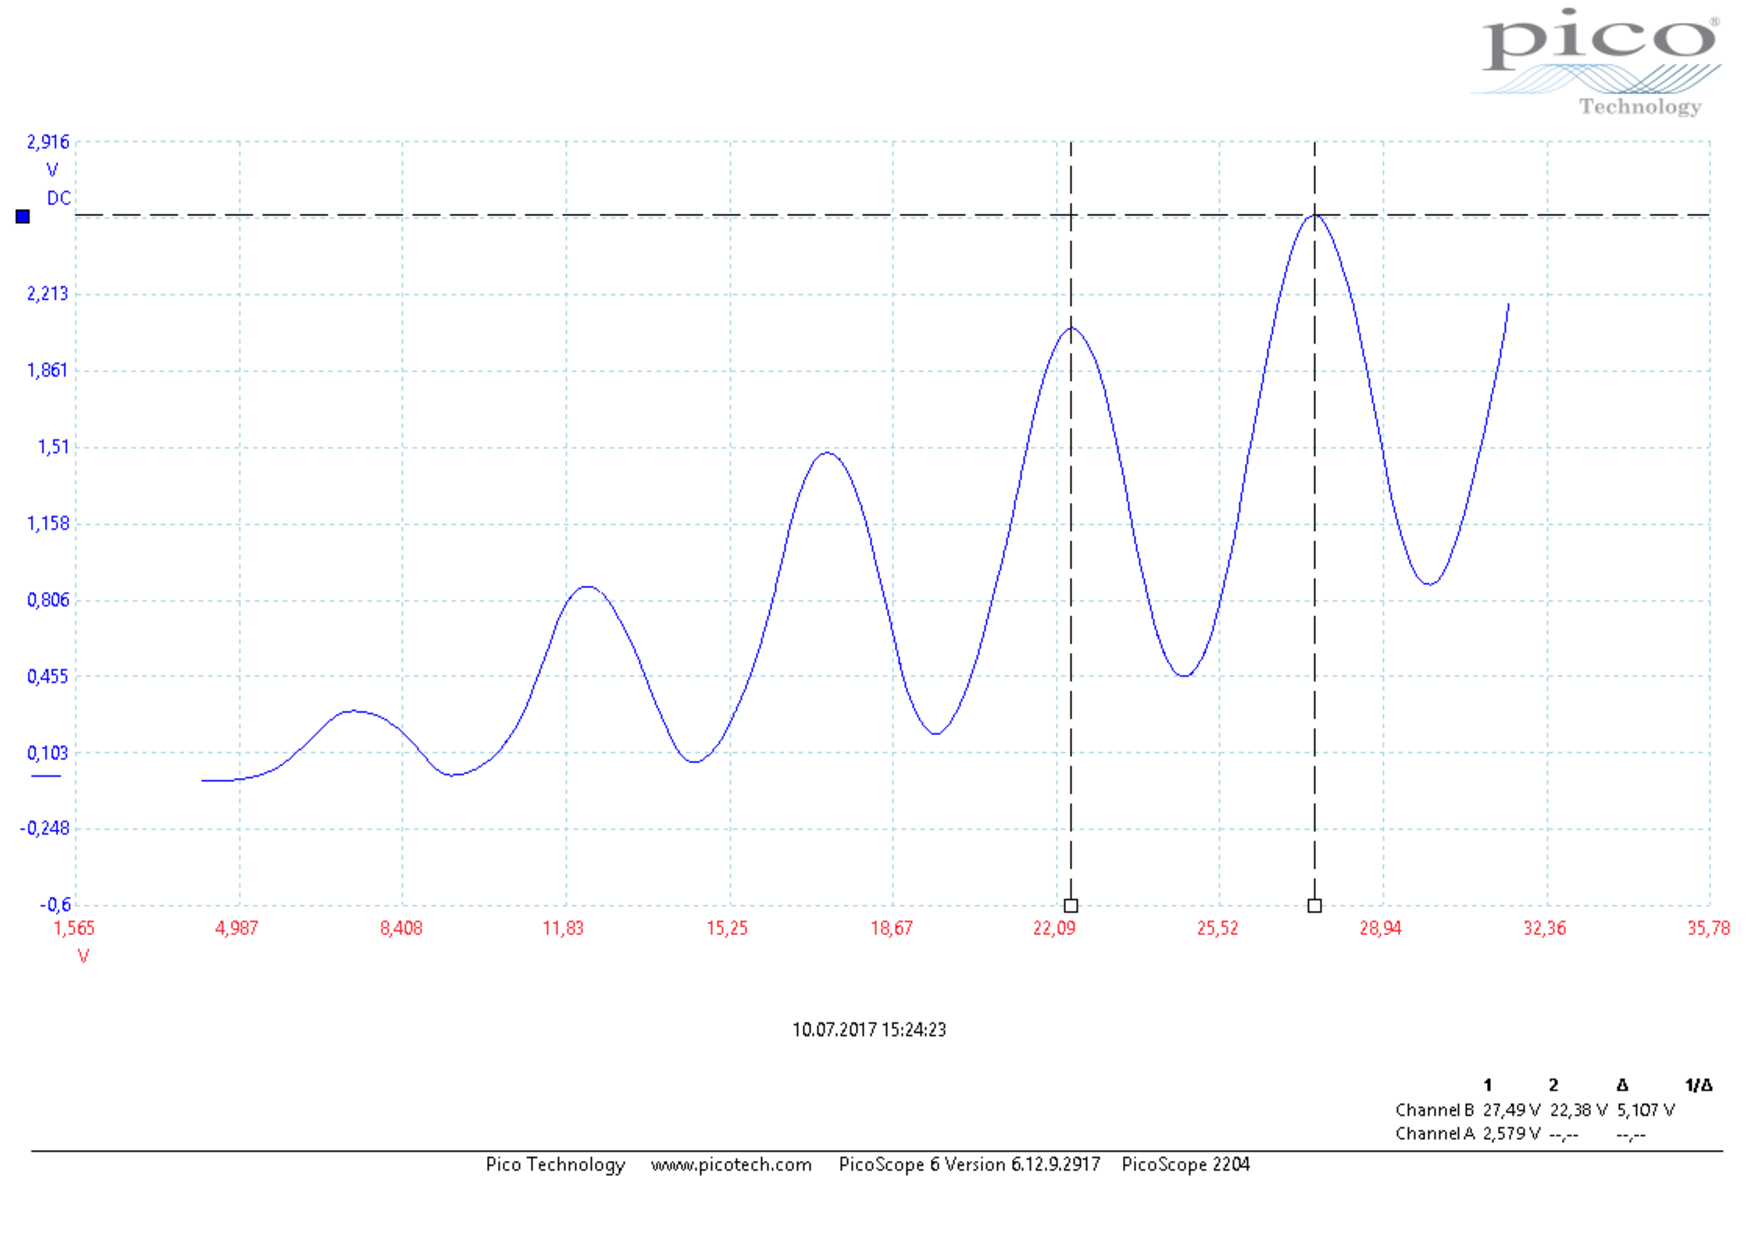
\includegraphics[width=\textwidth]{../Daten/Aufgabe1/Frank_Hertz_150.pdf}
	\caption{Franck-Herz-Kurve bei 150$ ^\circ $C}
\end{figure}
\begin{figure}
	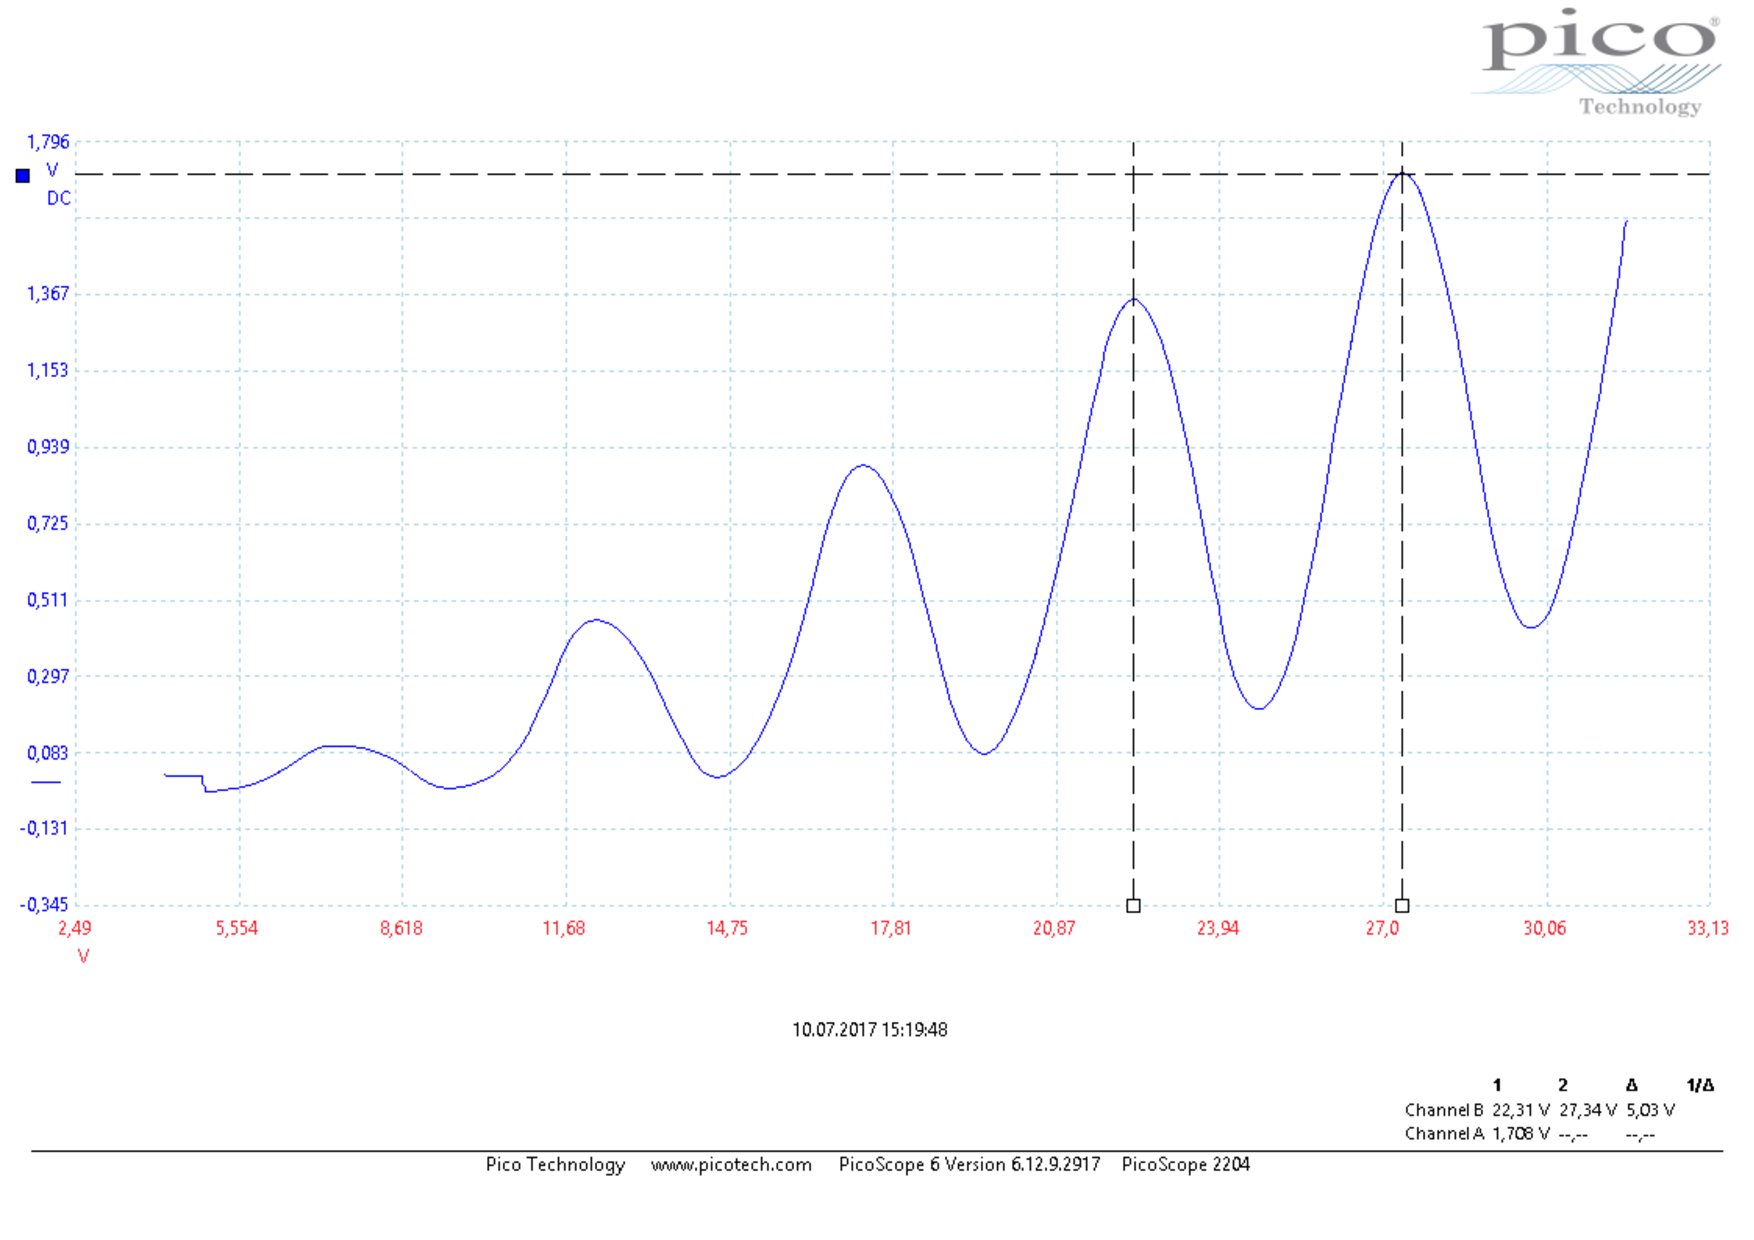
\includegraphics[width=\textwidth]{../Daten/Aufgabe1/Frank_Hertz_160.pdf}
	\caption{Franck-Herz-Kurve bei 160$ ^\circ $C}
	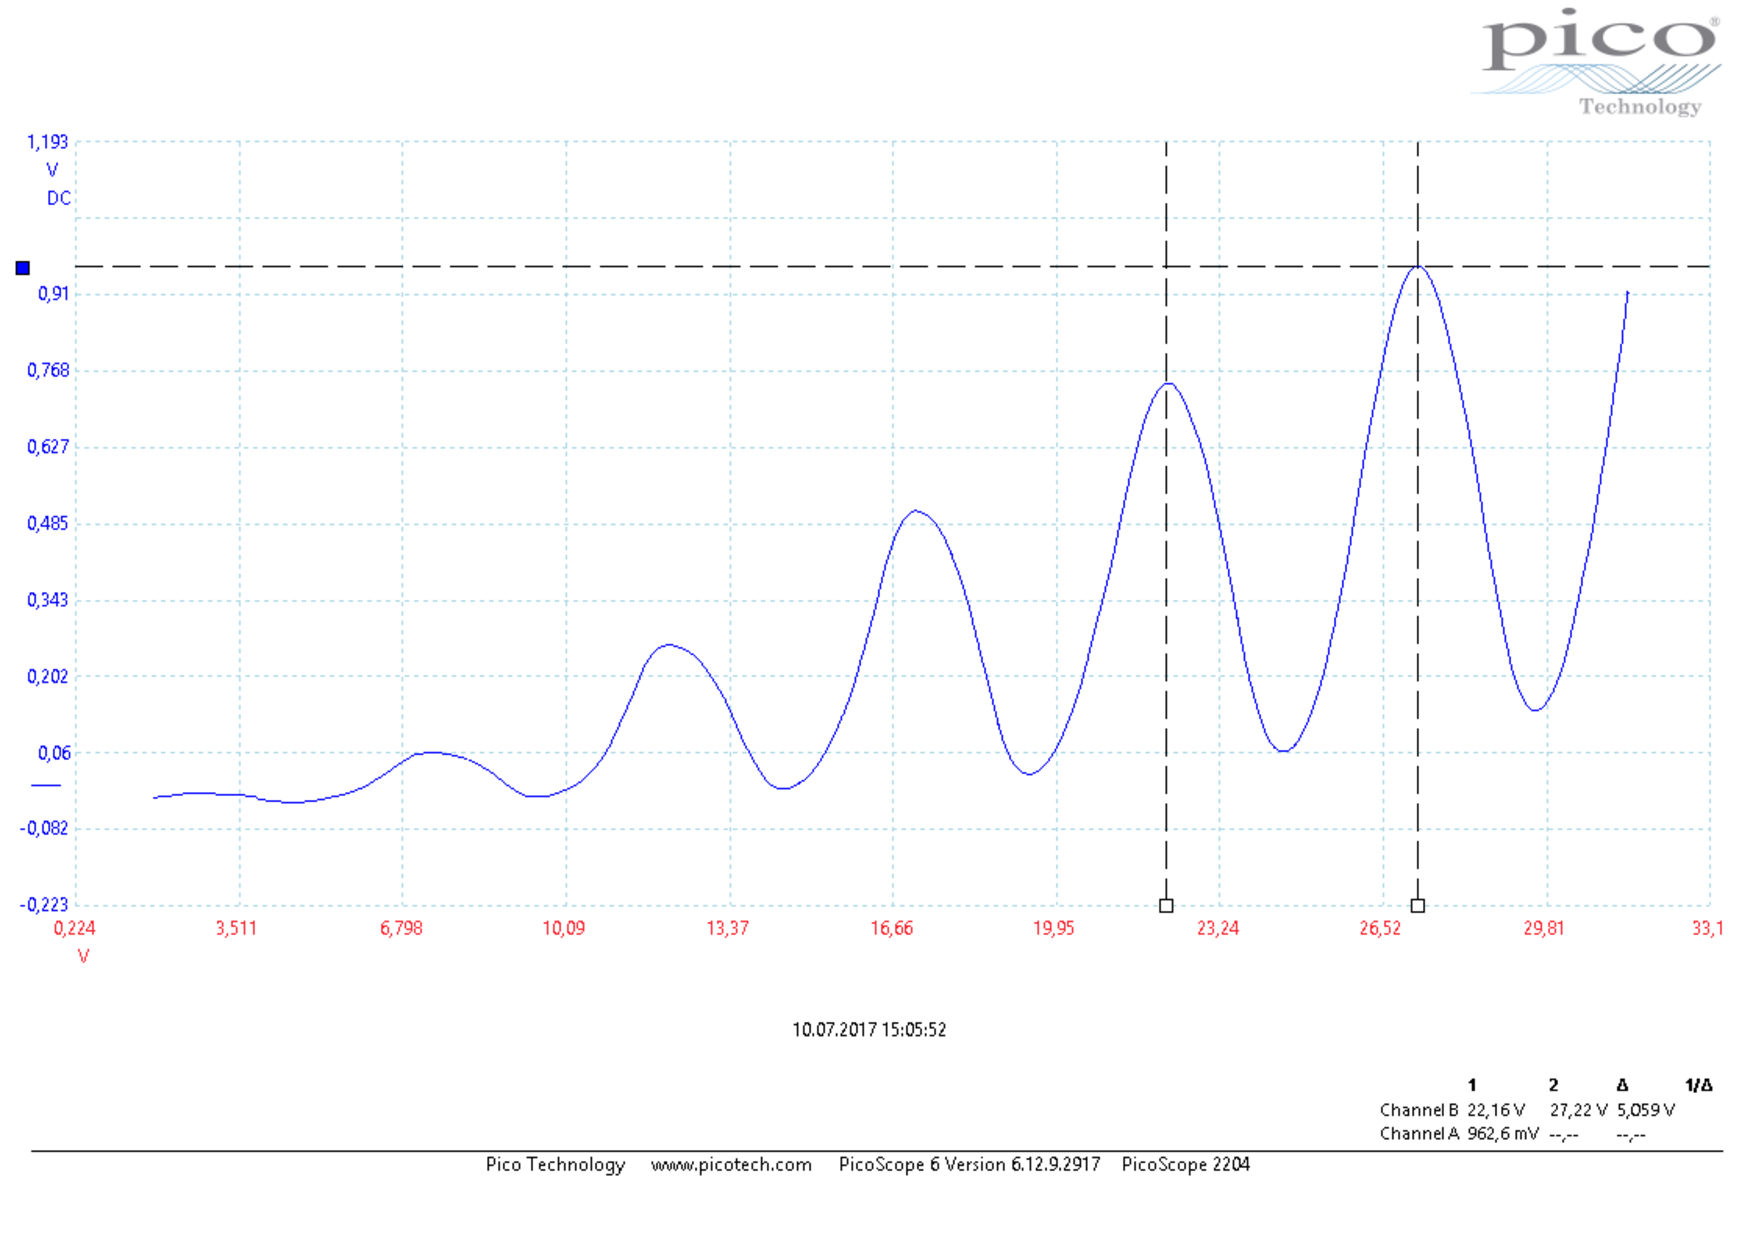
\includegraphics[width=\textwidth]{../Daten/Aufgabe1/Frank_Hertz_170.pdf}
	\caption{Franck-Herz-Kurve bei 170$ ^\circ $C}
\end{figure}
Somit erhalten wir die jeweiligen Thermospannungen über die Formel
\begin{align*}
U_{Th}=U_{n}+U_{1}-n\cdot \overline{\Delta U}\text{,}
\end{align*}
Hierbei ist $ \overline{\Delta U} $ der gemittelte Wert der $ \Delta U $ und $ U_{n} $ die Spannung des n-ten Peaks.

Aus diesen Werten erhalten wir nun den gemittelten Wert $ \overline{U_{th}} =6,407\; $V.
\begin{table}
	\centering
	\caption {Thermospannung in Abhängigkeit der Temperatur}
	\begin{tabular}{|c|c|}
		\hline
		Temperatur in $^\circ$C & U$_{th}$ in V \\ \hline
		170           &     6,379     \\ \hline
		160           &     6,381     \\ \hline
		150           &     6,294     \\ \hline
		140           &     6,553     \\ \hline
		120           &     6,427     \\ \hline
	\end{tabular} 
\end{table}
\section{Das Raumladungsgesetz}
Nun überprüfen wir das Raumladungsgesetz bei einer Temperatur von 120 $ ^\circ $C. Wir erwarten einen Zusammenhang der Form $I\propto U_{2}^{3/2}  $, weswegen wir die Messdaten wie folgt fitten
\begin{align*}
\log(I)=a\cdot \log(U_{2})+b\text{.}
\end{align*}
\begin{figure}
	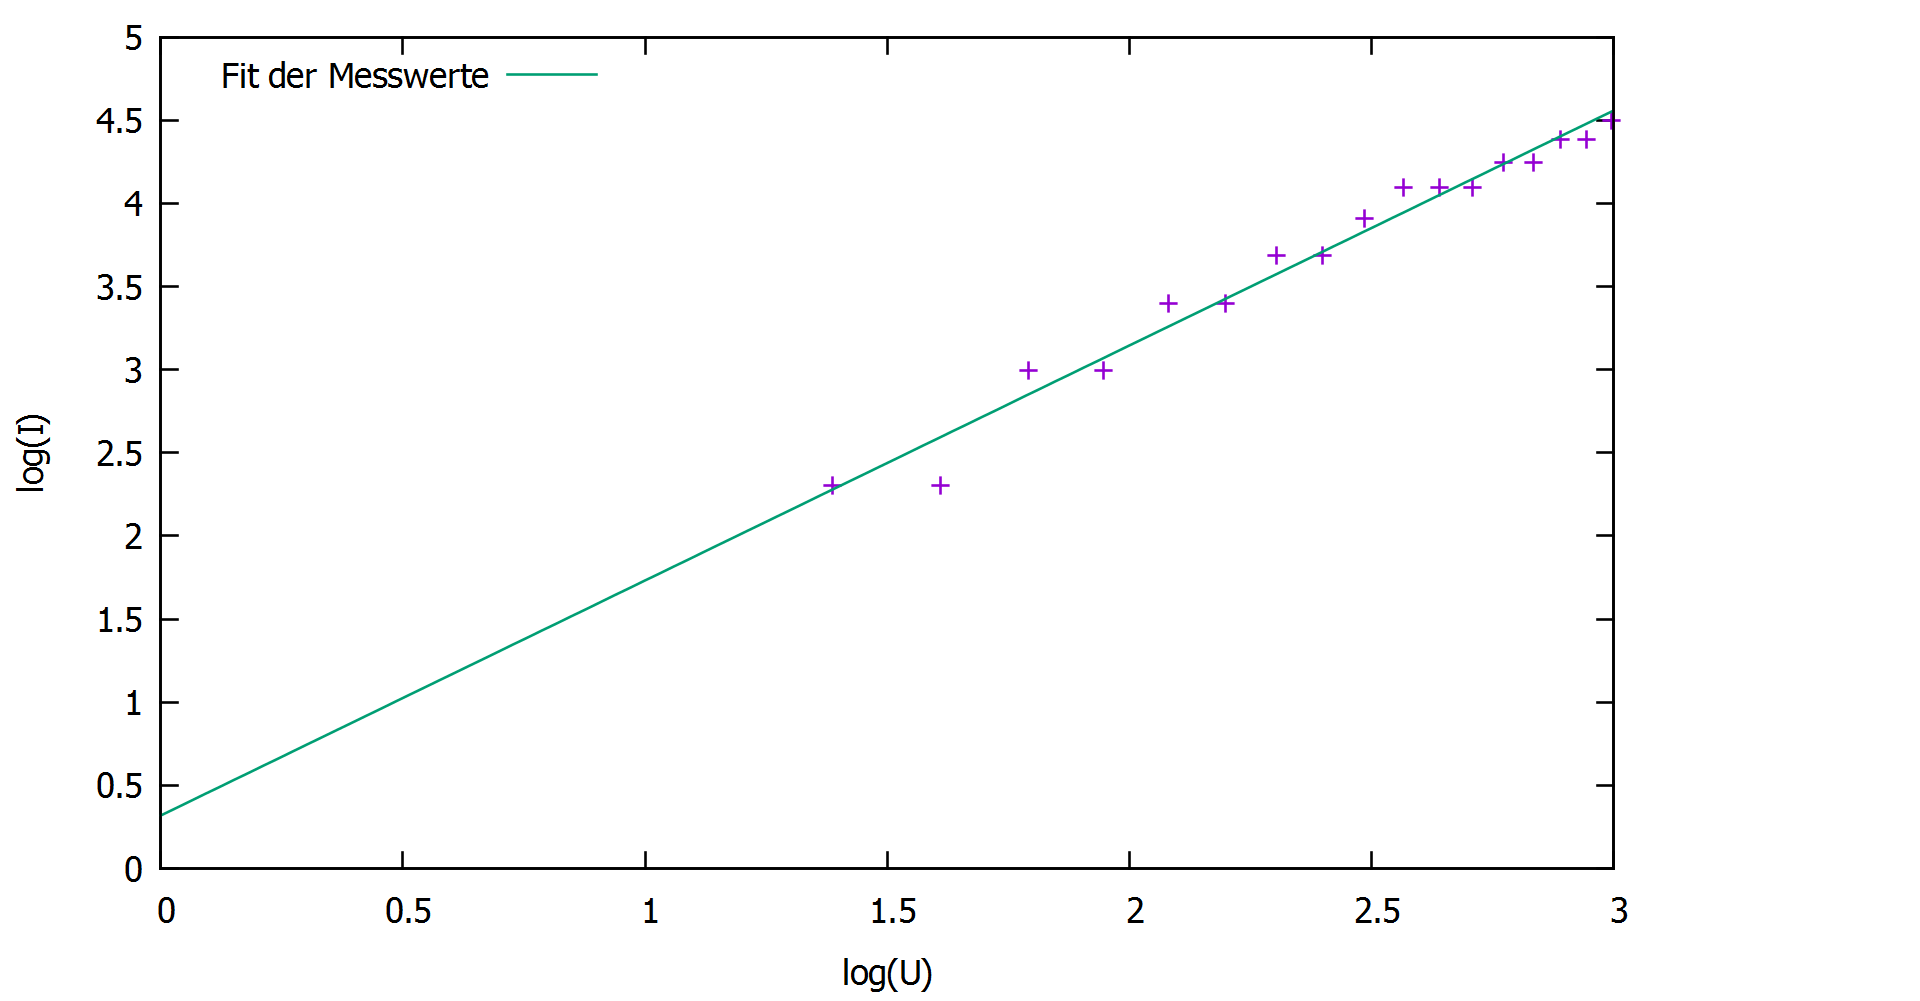
\includegraphics[width=\textwidth]{../Daten/Aufgabe1/Aufgabe1_3.png}
	\caption{Lineare Regression zu Kapitel 1.3 in Form von log(I)=a$ \cdot $log(U$ _2 $)+b}
\end{figure}
Die mit Gnuplot erstellte Funktion hat die Steigung a=1,414. Vergleicht man dies mit dem erhofften Wert(1,5) erhält man einen Fehler von 5,7\%.

\section{Ionisationsarbeit}
Nun wollen wir die Ionisationsarbeit von Quecksilber bei 120 $ ^\circ $C bestimmen.
\subsection{Bestimmung durch Graphische Ermittelung des Anstiegspunkts}
Zunächst bestimmen wir die Ionisationsarbeit indem wir die Stromstärke I$ _{in} $ über die Spannung U$ _2 $ auftragen und zwei Geraden durch die Messpunkte legen. Der Schnittpunkt der Geraden beschreibt dann den Anstiegspunkt und damit die Ionisationsarbeit. Hierbei stellt sich jedoch heraus, das einige Werte zu stark von der Form einer Geraden abweichen, weswegen diese Messpunkte vernachlässigt wurden. 
\begin{figure}
	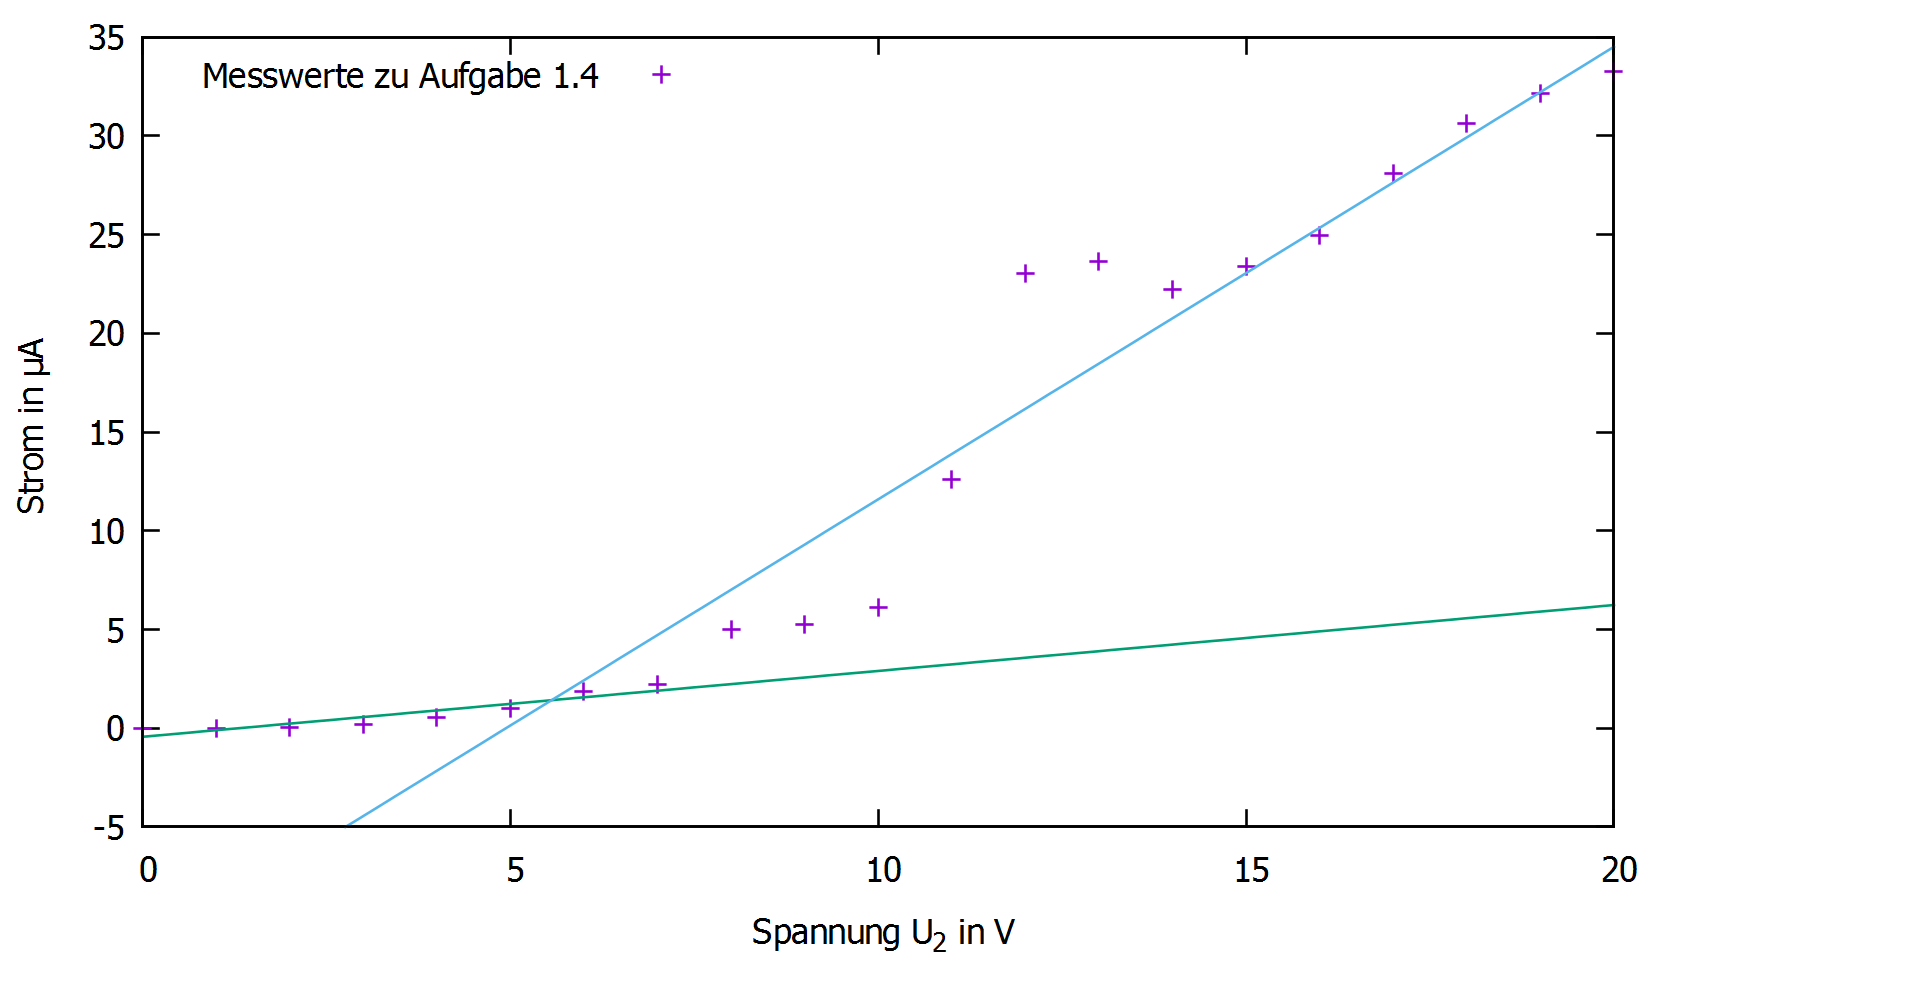
\includegraphics[width=\textwidth]{../Daten/Aufgabe1/Aufgabe1_4.png}
	\caption{Fit der Messwerte zu Aufgabe 1.4.1}
\end{figure}

Der Schnittpunkt befindet sich bei U$ _2 $= 5,579 V. Verrechnen wir nun noch die Thermokontaktspannung aus Kapitel 1.1 erhalten wir die Ionisationsarbeit 11,986 eV. Dies entspricht einer Abweichung vom Literaturwert (10,44 eV) von 12,9\%. Wir vermuten, dass dieser Fehler aufgrund von nicht beachteten Umständen während der Versuchsdurchführung entstand, da die gemessenen Werte ebenfalls sehr ungewöhnlich aussehen.
\subsection{Bestimmung über Auffängerspannung}
\begin{figure}
	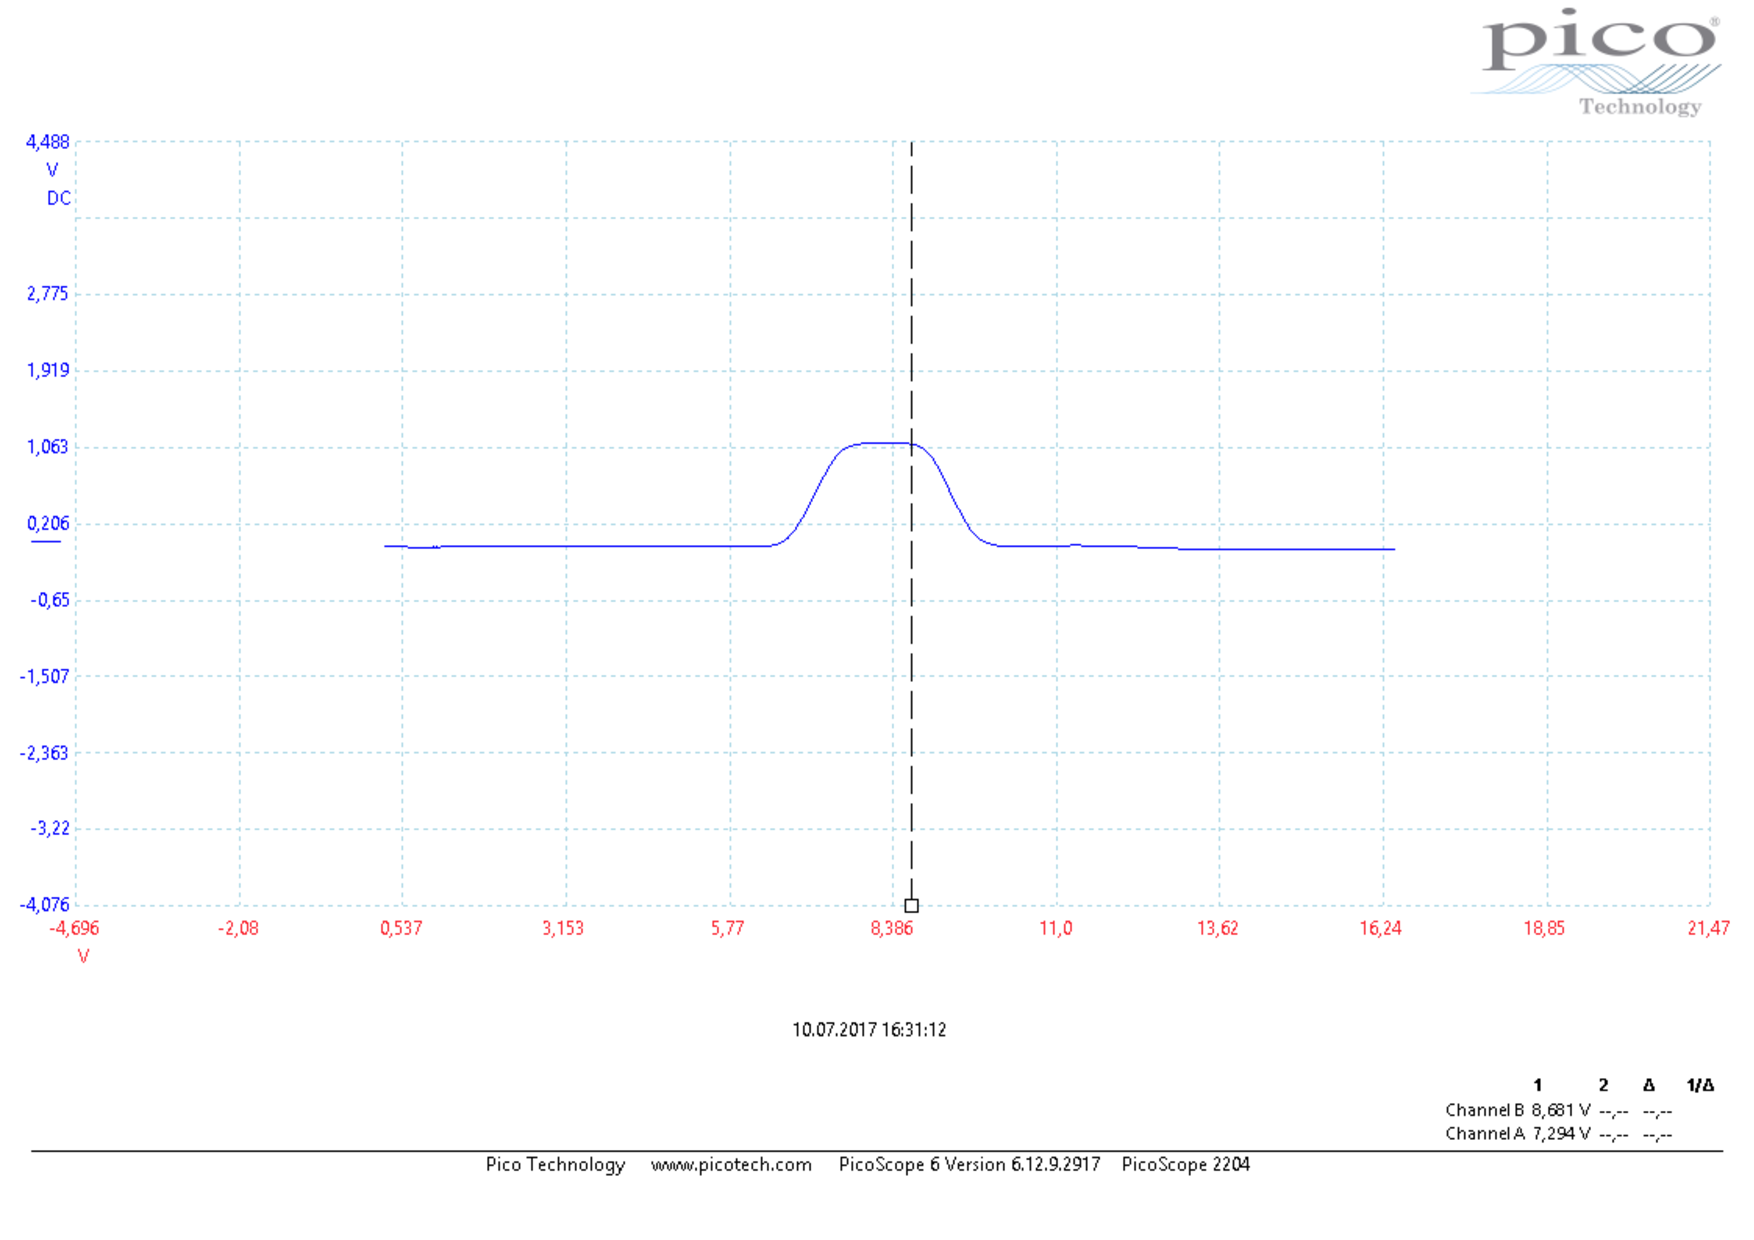
\includegraphics[width=\textwidth]{../Daten/Aufgabe1/Frank_Hertz_1_4_b_2.pdf}
	\caption{Auffängerspannung über Beschleunigungsspannung zu Aufgabe 1.4.2}
\end{figure}
Als zweite Variante wurde die Spannung direkt aus der im Graphen ablesbaren Auffängerspannung ermittelt, wobei dieser ebenfalls Ungewöhnlich aussieht. Mit dieser Methode erhalten wir eine Ionisationsarbeit von 10,789 eV, was einem Fehler von 3,2\% entspricht.
\section{Emissionsspektrum der Gasentladung}
Als letztes betrachten wir die Gasentladung mithilfe eines Taschenspektroskops. Hierbei konnten wir die Farben Rot, Gelb, Grün und Lila erkennen. Es ist möglich, dass es noch weitere sichtbare Farben gab, die wegen angelassenem Raumlicht nicht erkennbar waren.
